%--------------------------------------
% Create title frame
\titleframe

%--------------------------------------
% Table of contents
\begin{frame}{Sommaire}
  \setbeamertemplate{section in toc}[sections numbered]
  \tableofcontents[hideallsubsections]
\end{frame}

%==============================================
\section{État de l'art}
%==============================================

\subsection{Voxelization}

\begin{frame}[fragile=singleslide]{\insertsectionhead}
  \framesubtitle{\insertsubsectionhead}
    \textbf{Exemple d'utilisation:}
    \begin{itemize}
      \item Modélisation
      \item Simulation physique
        \begin{itemize}
          \item De nouvelles simulations rendues possibles
        \end{itemize}
      \item Eclairage volumétrique
    \end{itemize}

\end{frame}

%==============================================
\section{Etude de l'article}
%==============================================

\subsection{3D voxelization ? scanlines ?}

\begin{frame}[fragile=singleslide]{\insertsectionhead}
  \framesubtitle{\insertsubsectionhead}
\end{frame}

%--------------------------------------
\subsection{Spécificité de l'algorithme}

\begin{frame}[fragile=singleslide]{\insertsectionhead}
  \framesubtitle{\insertsubsectionhead}
  \begin{figure}[ht!]
    \begin{subfigure}{0.6\textwidth}
      \frame{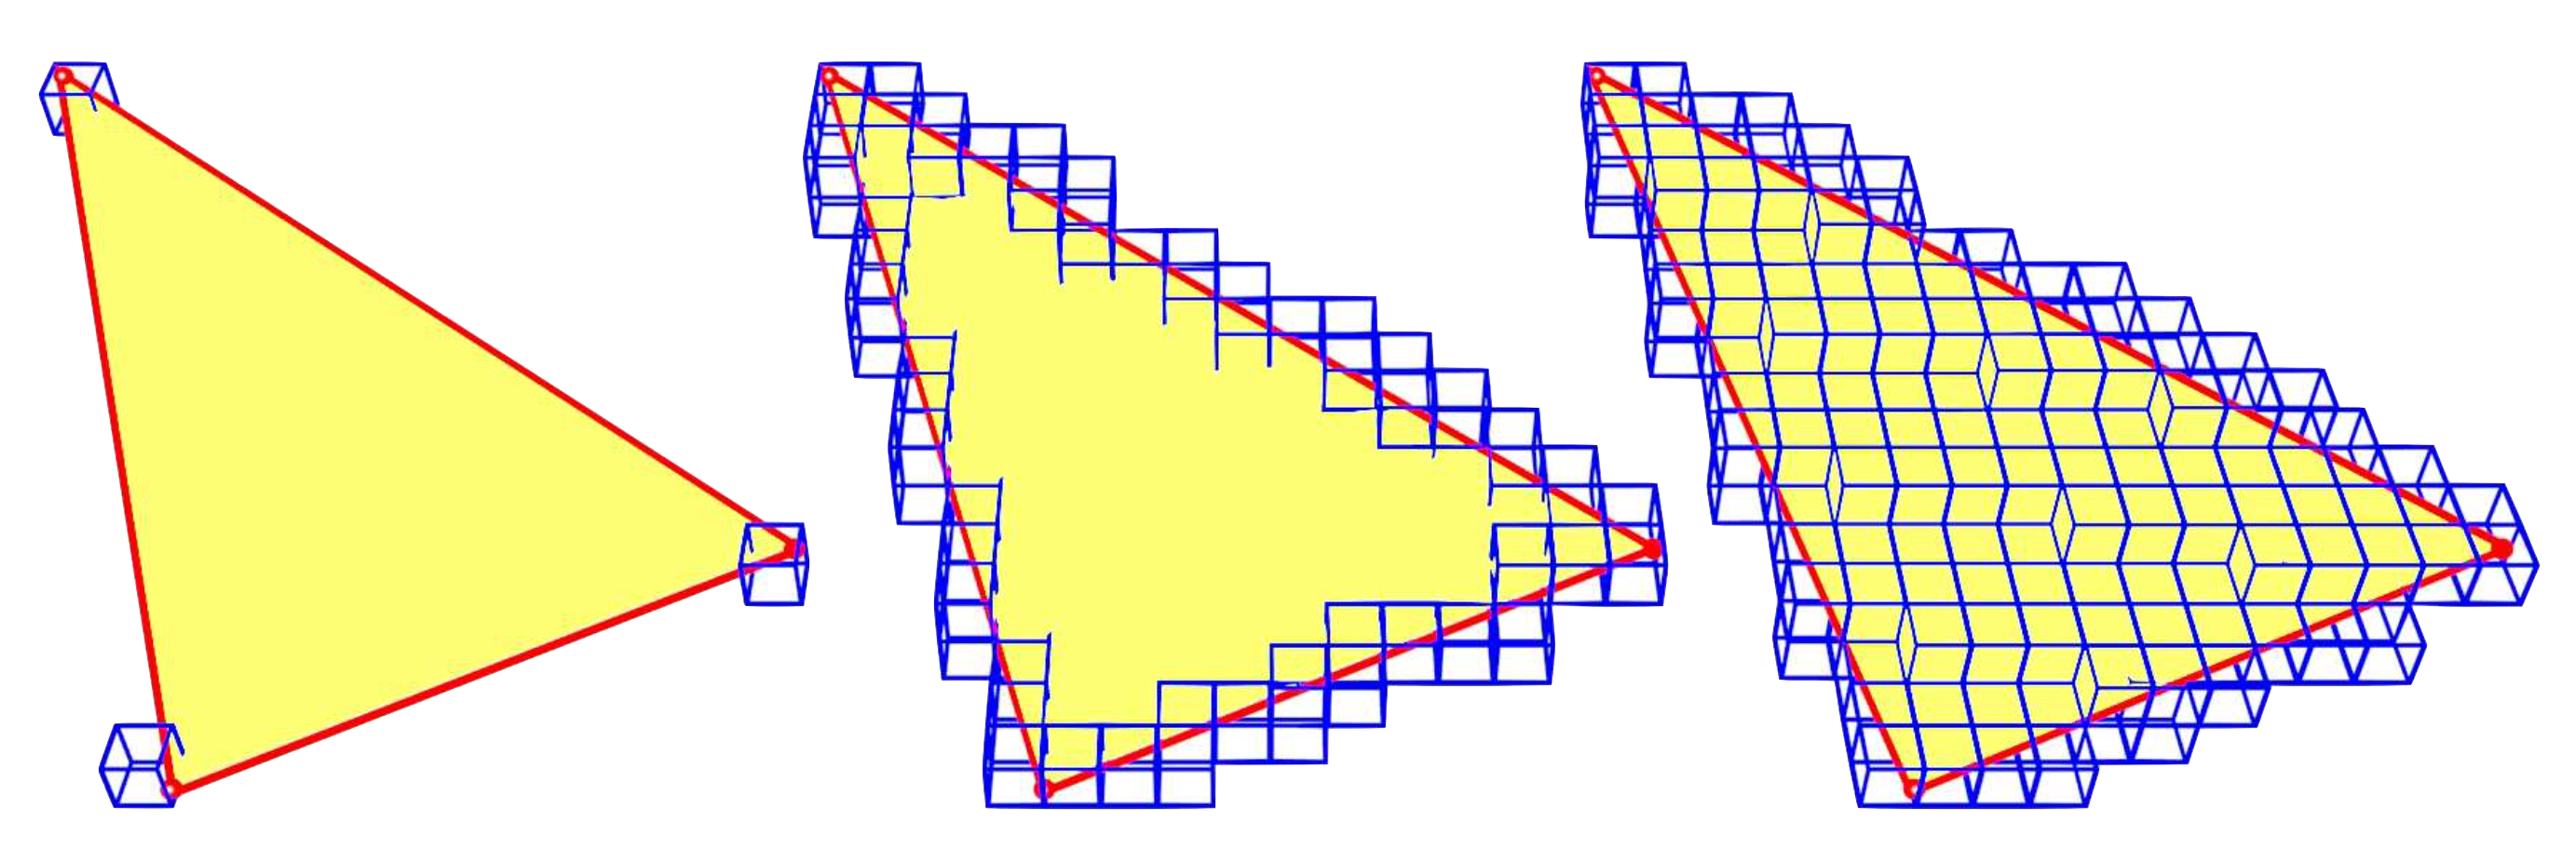
\includegraphics[width=\textwidth]{resources/voxelization_steps.png}}
      \caption*{Etapes de la voxelization}
    \end{subfigure}
    \hfill
    \begin{subfigure}{0.2\textwidth}
      \frame{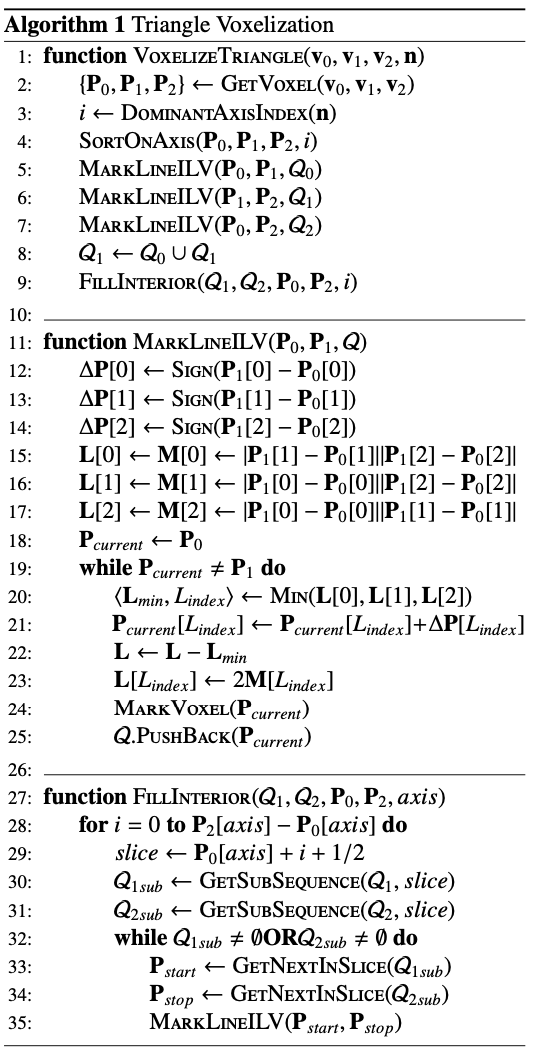
\includegraphics[width=\textwidth]{resources/algo_paper.png}}
    \end{subfigure}
  \end{figure}
\end{frame}

%--------------------------------------
\subsection{Points clés}

\begin{frame}[fragile=singleslide]{\insertsectionhead}
  \framesubtitle{\insertsubsectionhead}
  \begin{itemize}
      \item Très rapide
      \item Parfaitement compatible avec le multithreading
      \item Plus on a de triangles plus c'est rapide
      \item L'approximation des entiers réduit les trous dans la couverture
    \end{itemize}
    \vfill
    \begin{figure}
      \begin{subfigure}{1\textwidth}
        \frame{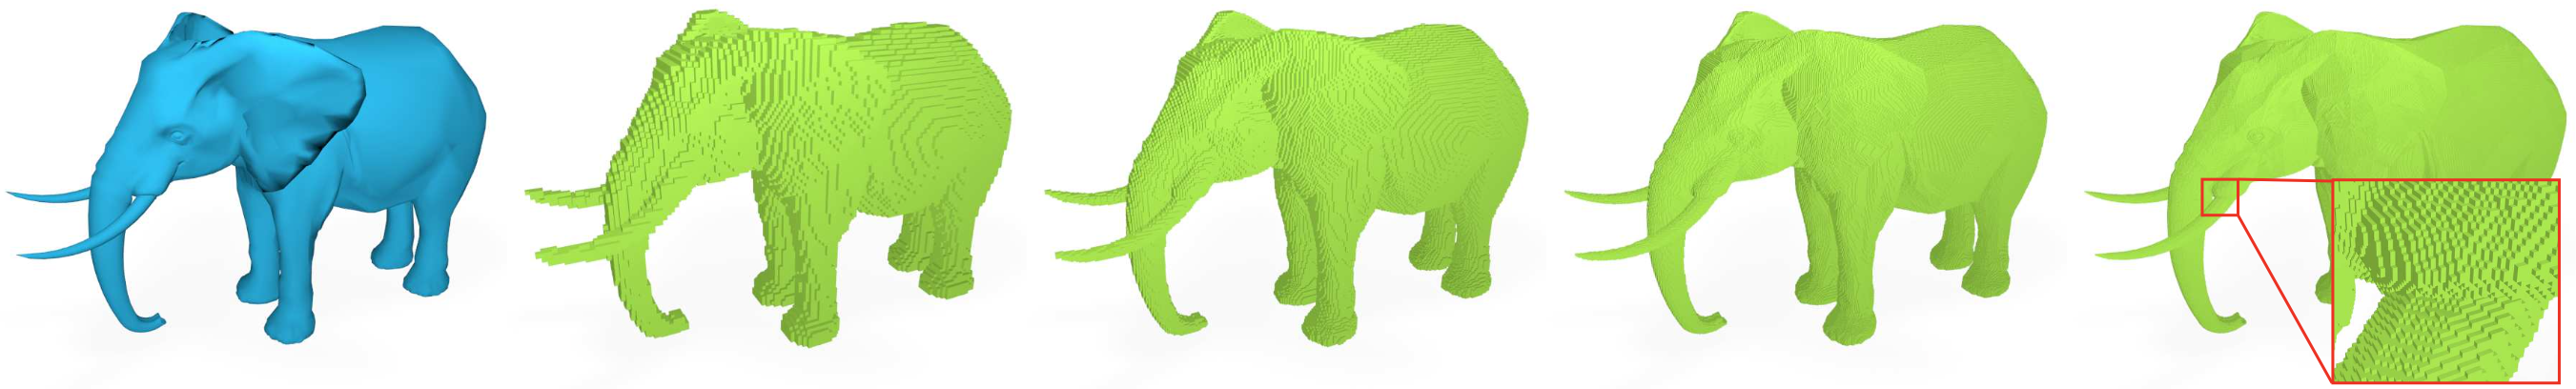
\includegraphics[width=\textwidth]{resources/elephant.png}}
      \end{subfigure}
    \end{figure}
    
    
\end{frame}

%==============================================
\section{Prototypage}
%==============================================

\subsection{Notre plan initial}

\begin{frame}[fragile=singleslide]{\insertsectionhead}
  \framesubtitle{\insertsubsectionhead}
\end{frame}

%--------------------------------------
\subsection{Premiers jours}

\begin{frame}[fragile=singleslide]{\insertsectionhead}
  \framesubtitle{\insertsubsectionhead}
\end{frame}

%--------------------------------------
\subsection{Difficultés rencontrées}

\begin{frame}[fragile=singleslide]{\insertsectionhead}
  \framesubtitle{\insertsubsectionhead}
\end{frame}

%--------------------------------------
\subsection{Éclaircissement des zones d'ombres sur l'article}

\begin{frame}[fragile=singleslide]{\insertsectionhead}
  \framesubtitle{\insertsubsectionhead}
\end{frame}

%==============================================
\section{Résultats \& Benchmark}
%==============================================

\subsection{Quelques chiffres en comparaison}

\begin{frame}[fragile=singleslide]{\insertsectionhead}
  \framesubtitle{\insertsubsectionhead}
\end{frame}

%--------------------------------------
\subsection{Démo}

\begin{frame}[fragile=singleslide]{\insertsectionhead}
  \framesubtitle{\insertsubsectionhead}
\end{frame}

%--------------------------------------
\subsection{Perspectives d'évolution}

\begin{frame}[fragile=singleslide]{\insertsectionhead}
  \framesubtitle{\insertsubsectionhead}
\end{frame}

%--------------------------------------
\subsection{Conclusion}

\begin{frame}[fragile=singleslide]{\insertsectionhead}
  \framesubtitle{\insertsubsectionhead}
\end{frame}

